\chapter{Introduction}
\label{chapter:intro}
\epigraph{\textit{So kaputt kriegst du mich nie, das schaff ich nur ganz alleine}}{Von Wegen Lisbeth}

\section{Thin liquid films}
Thin liquid films appear in multiple forms. 
We find them in ordinary situations such as washing our hands, where a thin water layer adheres to our skin. 
Another example can be found inside fully automatic coffee machines.
In the inner tubs of these machines coffee grounds are mixed with hot water to brew coffee. 
Small amounts of this mixture stays inside the tubes covering them with a thin film.
This film serves as nutrient rich ``glasshouse'' to bacteria and spores, which inevitably leads to the growth of a so called biofilm, making it necessary to clean them regularly.
The bacteria in these biofilms actually often produce enzymes which effectively reduce the surface tension, thus a biofilm is often an active thin film. 
Of course, some thin film phenomena will be explained in a more detailed manner throughout this thesis. 
A visual representation of some thin film flows can be found in Fig.~\ref{fig:examples_intro}.
\begin{figure}
    \centering
    \includegraphics[width=0.95\textwidth]{graphics/Three_tile_intro_smaller.png}
    \caption{Illustrative examples of thin film flows. 
    In (a) rain drops seem to choose random paths running down a window, during their motion they leave behind smaller drops which is called pearling. 
    Tile (b) displays the interaction between water and a plant leaf. 
    Drops are formed quickly and due to the curvature of the leaf's surface the coalescence of droplets is enhanced. 
    Soap bubbles are a prime example of a thin film flow, as shown in (c). 
    A small amount of liquid is enclosed between two gas phases. Inside the film fluid is drained to the bottom of the bubble due to gravity.}
    \label{fig:examples_intro}
\end{figure}

To describe thin film problems, however, one has to start somewhere.
And the starting point for me and this thesis was to learn about the governing equations of fluid dynamics. 
Those equations are called the Navier-Stokes equations and they resemble the dynamics of a fluid constraint due to several symmetries~\cite{Navier, Stokes}, e.g., conservation of mass and momentum.
Solving these equations in a strict mathematical manner, therefore showing existence and smoothness of a solution is an elusive quest. 
Although being around for roughly two centuries this equation\footnote{Strictly speaking the Navier-Stokes equation is a momentum equation, however it is often accompanied with an continuity equation.} is one of the seven problems which are considered to be worth a million dollars when solved. 
The collection of these problems is called ``Millenium problems'' and the Navier-Stokes equation poses one of the six unsolved problems.
A quality that differentiates physics from mathematics is the understanding of an approximation.
While it is true that we cannot strictly solve the Navier-Stokes equation, we still have a rather good understanding due to well working approximations.
This statement is supported by the constant innovation in computing techniques and, more so, computing hardware. 
Todays algorithms are able to \textit{brute force} an approximate solution to a wide class of problems.  
Some examples to be named are the air flow around an airfoil or the catamaran boat structure to reduce drag. 
The main topic of my work, however, is the dynamics of thin liquid films which admits a crucial simplification to the Navier-Stokes equation. 
Nevertheless it should be noted that theoretical and computational fluid dynamics (CFD) is by all means a complex but also a vibrant and constantly evolving field.

Generally there are three paths to study the dynamics of thin liquid films.
One can work with the partial differential equations and derive the dynamics from them. 
This is the theoretical approach which uses analytical calculus to derive solutions.
On the other hand it is possible to study fluid dynamics with experiments.
Studying thin film flows by experiments can be a tedious task.
Although the experimental system is quite approachable, a thin liquid layer on a substrate, the devil lies in the details.
Preparation of films with uniform thickness of only a few nanometers is not a trivial task.
Measurements are often a series of images with frame rates that allow to document dynamics in the region of $\approx 10^{-5}$ seconds.
This series of images or other control parameters allow then to derive results from observations.
Both however, theory as well as the experiment, have shortcomings. 
Theoretical assumptions can be wrong or the resulting system of equations can be too complex to be solved. 
Experiments often do not allow for the very fine grained control and independent change of different parameters.
The third approach, which is used throughout this thesis lies in between the experiment and a purely theoretical one.
Numerical modelling or computational fluid dynamics allows to approximate the complicated partial differential equations while also allowing for fine grained parameter studies.

To study thin films and in the end to write this thesis I had to broaden my understanding of (numerical) modelling. 
Which solver, algorithms and simplifications are used in common fluid dynamics research?
How do they compare with each other and which of those are relevant for the model I used and developed? 
I had to learn about algorithms and numerical techniques and among them I focused on the lattice Boltzmann method(LBM)~\cite{benziLatticeBoltzmannEquation1992a, chenLatticeBoltzmannMethod1998, heTheoryLatticeBoltzmann1997, guoDiscreteLatticeEffects2002, krugerLatticeBoltzmannMethod2017}.
I also learned how approachable the thin film research can be. 
Whenever some liquid is pushed onto a dry surface, for example watercolor on a white canvas, thin film theory can help to shine light on the distribution of paint~\cite{thielePatternedDepositionMoving2014, oronLongscaleEvolutionThin1997, edwardsNotSpreadingReverse2016}. 
At some point in our life most of us watched rain drops run down a transparent window~\cite{wilczekSlidingDropsEnsemble2017}, as shown in Fig.~\ref{fig:examples_intro}a. 
The question of why a drop chooses its very own path has a lot to do with the window's surface topology and the three phase contact line (TPC) of the droplet~\cite{cassieWettabilityPorousSurfaces1944, suzukiSlidingBehaviorWater2008, liuActuatingWaterDroplets2015}. 
Why do droplets form at all, e.g.,  after a foggy morning, can be studied in the framework of the thin film equation as well~\cite{zhangInkjetPrintingDirect2015, shiFogHarvestingHarps2018}.
Although these phenomena happen in many situations their theoretical understanding is far from being complete.
Just to highlight one of the above-mentioned situations, the wetting of a dry surface is a highly sophisticated problem.
Using the thin film equation as a mathematical model comes short in explaining the wet-dry transition.
Even worse, to move the liquid on top of a dry surface one would need an infinite amount of energy.
This has to do with boundary conditions and is called the \textit{Huh-Scriven paradox}, which states: ``Not even Herakles could sink a solid if the physical model were entirely valid''~\cite{huhHydrodynamicModelSteady1971}.
In fact, the quote has to be understood in two ways. 
First and foremost, the thin film equation is a powerful tool in modelling a lot of fluid dynamics problems.
Second is the criticism on the rough approximations, i.e., about the \textit{no-slip} boundary condition, which requires a vanishing flow velocity at the substrate.
Of course, nature finds a way around and does not use infinite amounts of energy to make a droplet slide. 
In the end the \textit{no-slip} boundary condition is just a model.
Definitely one of the better models, but one that comes short of explaining wetting sufficiently well.

In the following chapters of this thesis I discuss what kind of problems can be modelled with approaches similar to the thin film equation.
Showing how broad the use cases are and where possible extensions can lead to.
Having these use cases, both academic and industrial, is of utmost importance to justify the further development of thin film models. 
Following this short illustrative part will be, of course, the introduction of the mathematical models with their partial differential equations (PDE). 
However, this is nothing more than an efficient way of describing the problem.
Strictly speaking mathematics as well as algorithms serve as tools not as the goal of this thesis. 
%Therefore, I try my best to keep it as simple as possible with analogies and hopefully self explaining figures.
Therefore, the \textbf{KISS} concept, keep it simple stupid, is one core concept that is used throughout.
Most mathematical models are accompanied with explenatory figures.        

\section{Selected applications of the thin film equation}
\label{section:applications}
\begin{figure}
    \centering
    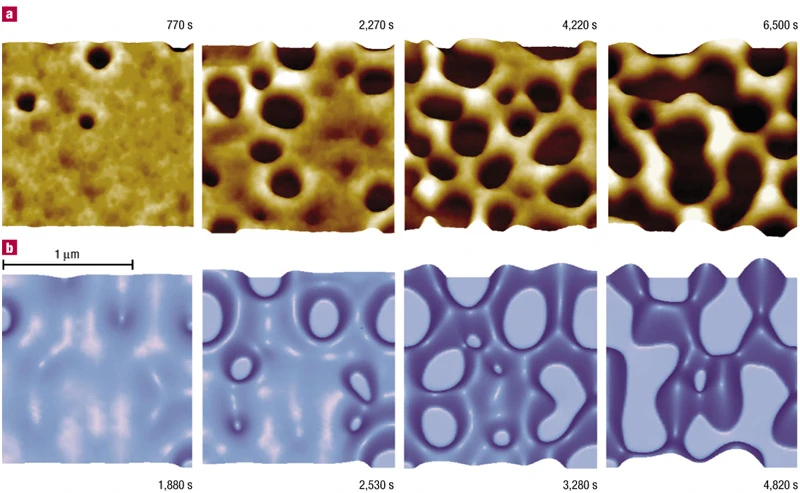
\includegraphics[width=0.75\textwidth]{graphics/41563_2003_Article_BFnmat788_Fig1_HTML.png}
    \caption{Film dewetting of a surface in the spinodial regime.
    Series (a) are experimental measurements with an AFM, while series (b) is generated using a numerical approach with the same parameters taken from~\cite{beckerComplexDewettingScenarios2003}.}
    \label{fig:becker_dewetting}
\end{figure}
Applications of the thin film equation cover a wide range of use cases. 
There is for example the problem of pesticide distribution in agriculture, a problem that requires that the pesticide sticks to the plant.
From a medical perspective, our lung and in particular the alveoli need to be covered with a thin film with a well defined concentration of biological surfactants~\cite{hermansLungSurfactantsDifferent2015}.
Certain diseases inhibit the surfactant production and therefore threaten partial or full collapse of the lung~\cite{doi:10.1146/annurev.fl.26.010194.002525}.

Coatings of surfaces are one of the problems that has been scientifically investigated for the last few decades.
There are various ways to coat a surface with arbitrary kinds of liquids.
What is common to all of them is the fact that the process heavily relies on the affinity between the to be coated surface and the coating agent~\cite{bonnWettingSpreading2009}.
If this affinity is too small the coating is unstable and therefore making the film prone to wrinkling~\cite{dasilvasobrinhoStudyDefectsUltrathin1999} or eventually even rupture~\cite{oronLongscaleEvolutionThin1997, crasterDynamicsStabilityThin2009, beckerComplexDewettingScenarios2003}, as shown in Fig~\ref{fig:becker_dewetting}.

\begin{figure}
    \centering
    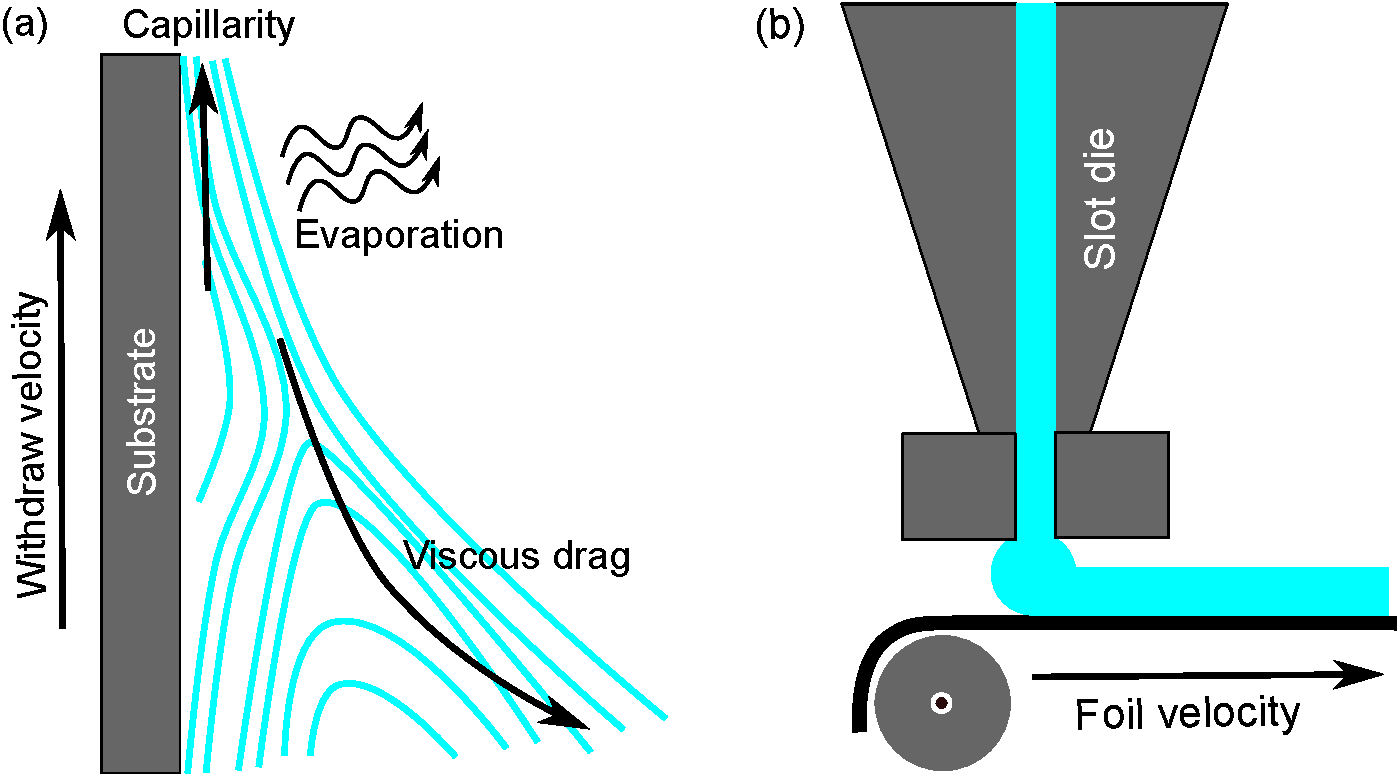
\includegraphics[width=0.75\textwidth]{graphics/Coating_intro.pdf}
    \caption{(a) Schematics of the dip coating process. 
    A substrate is withdrawn from a fluid bath and due to capillarity and solid-liquid interactions (adhesion) some liquid adheres to the substrate.
    Balancing between adhesion and viscous drag most of the liquid is left in the bath.
    Depending on the surface tension and atmospheric pressure, evaporation can further thin the drawn film.
    (b) Schematics of a slot die coating process.
    A die is placed on top of a constantly moving foil.
    Through that die a liquid is pumped onto the moving foil.}
    \label{fig:dip_coating}
\end{figure}
For different length scales (m, cm, mm) and for different materials (metals, glasses, polymer compounds) there exist different coating approaches.
The industrial coating process of a five by five meter aluminium plate differs significantly from the process to coat a millimetric biological sensor.
Among the various coating approaches one is the so-called dip coating process, as displayed in Fig.~\ref{fig:dip_coating}(a). 
Much like the name suggests the to be coated object is dipped into a reservoir of coating liquid~\cite{scrivenPhysicsApplicationsDIP1988, darhuberSelectiveDipcoatingChemically2000, grossoHowExploitFull2011}.
While the process itself is straightforward the \textit{art} of dip coating is far from being trivial, meaning that this process requires tight tolerances on extraction velocity, material parameters and if possible a vibration free extraction.

From a theoretical point of view this problem has first been addressed by Landau and Levich ~\cite{landauDraggingLiquidMoving1988} as well as Derjaguin~\cite{derjaguinThicknessLiquidFilm1993}.
In their fundamental work they derived two limits concerning the dynamics of the film during the extrusion.
The low extrusion velocity limit assumes that gravity and as such inertia is small and can be neglected, at least for a simple plate geometry.
The resulting equation leads to a balance between capillary and viscous forces. 
The film that is drawn with the object is usually very thin and the resulting meniscus between the object and the fluid reservoir is in size proportional to the capillary length.
In fact the thickness of the coating film is roughly given as $h_{\infty} \propto l Ca^{2/3}$, where $l$ is the capillary length and $Ca$ the capillary number.
The capillary number $Ca$ is one among many non-dimensional numbers in fluid dynamics.
It compares viscous drag with surface tension, whereas the capillary length $l$ is a length scale that separates between gravity and capillary driven dynamics.
This can be understood simply by looking at droplets. 
As long as the volume is small the droplet will form a spherical cap.
If the volume becomes too large, a paddle will form with a distinct difference in shape from a spherical cap, because gravity can no longer be neglected.
In the converse limit of high extrusion velocity the capillary forces become subdominant.
Therefore viscous forces are being balanced with gravity. 
Using the same scaling argument as before the coating thickness can be approximated with $h_{\infty} \propto l Ca^{1/2}$.
Clearly these two regimes show that the extrusion velocity of the coated object has a significant impact, assuming that the surface tension and viscosity are constant parameters.

In case of die or slot die coating the to be coated object is not immersed into a reservoir of coating liquid.
Instead the coated material is usually an elastic foil which moves with constant velocity under a die.
A film is created because the coating fluid is pumped through the die which is placed on top of the foil with some distance $d$.
Similar to the illustration in Fig.~\ref{fig:dip_coating}(b), a film is drawn due to balance between capillary and viscous forces.
The thickness of the resulting film however does not depend on gravity in this case.
Ruschak showed that similar to the low extrusion velocity limit of the dip coating problem the film thickness after die coating can be approximated using $h_{\infty} = d~Ca^{2/3}$~\cite{ruschakLimitingFlowPremetered1976}.

These two examples highlight an important behaviour.
The solution consists of some variable, here the capillary number, that scales with a well defined exponent, e.g., $2/3$ in the low and $1/2$ in the high extrusion velocity scenario.
These results can be addressed as dimensional analysis, a rather fancy word for matching dimensions on both sides of the equation.
In the end the height or thickness needs to be of the dimension of a length.
They often support so-called self similar behaviour, meaning under change of one or more parameters it is possible to collapse data on a master curve. 
Another dynamic problem that exhibits self similar behaviour is droplet coalescence, which is shortly discussed in Chapter~\ref{chapter:fourth_paper} and liquid lens coalescence~\cite{hackSelfSimilarLiquidLens2020, scheelViscousInertialCoalescence2023}. 
% I am here
\section{Literature overview}
\label{section:literature}
\begin{figure}
    \centering
    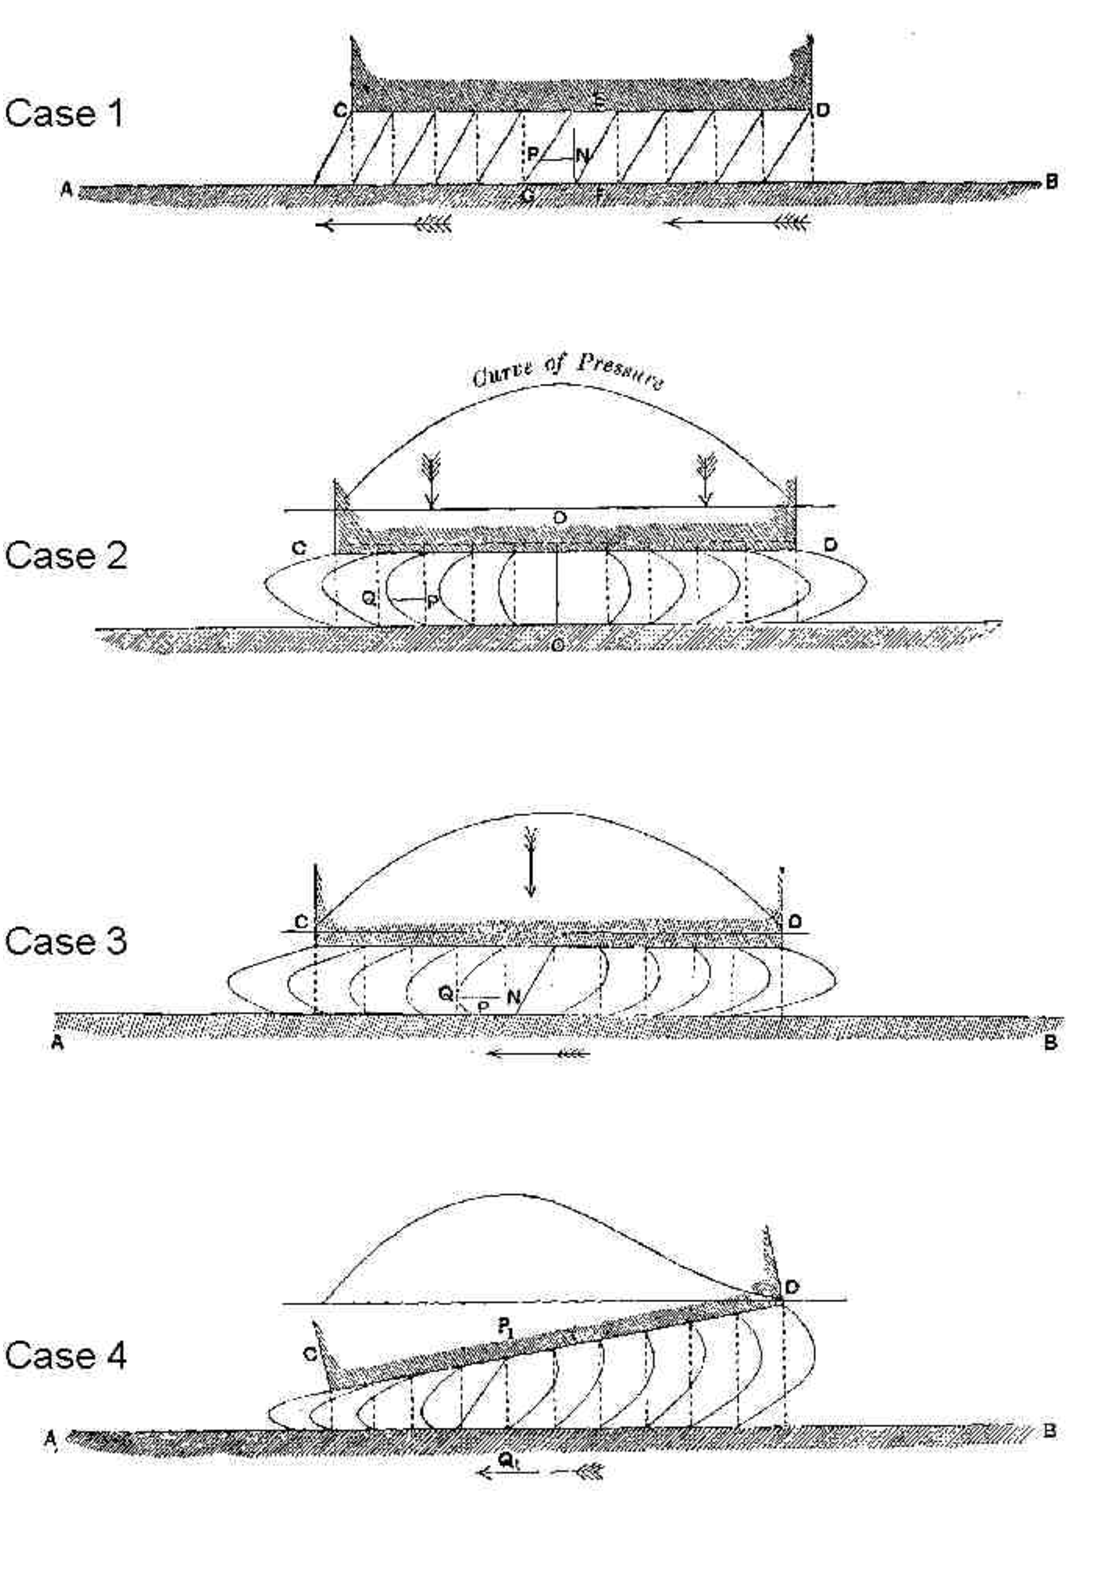
\includegraphics[width=0.85\textwidth]{graphics/reynolds_slip_bearing.pdf}
    \caption{A drawing from Osborn Reynolds on slipper bearing lubrication.
    The four figures are taken from Ref.~\cite{reynoldsTheoryLubricationIts1886} and cropped together in a single image.
    In (a) surface CD is fixed while surface AB moves to the left with velocity U. 
    The fluid between the surfaces feels the force $F = \mu \frac{U}{h}$, with $h$ being the separation distance.
    The velocity profile changes uniformly from $U$ at AB to zero at CD. 
    Panel (b) displays the case when two parallel surfaces approach each other.
    The pressure acting on surface CD is shown on top of the surface.
    Each line between the surfaces shows the tangential forces and thus indicates the fluid velocity profile.
    Allowing surface AB to move to the left while surface CD approaches with the same pressure distribution as in (b) it is shown in (c).
    This case is a combination of (a) and (b) with non-uniform force distribution between the surfaces.
    The last panel (d) displays the case when the surfaces are not parallel.
    Surface CD is kept constant while surface AB is moved to the left.
    The curve on top displays the pressure the fluid exerts on surface CD.}
    \label{fig:reynolds_work}
\end{figure}
Fluid dynamics in general is mathematically described by the Navier-Stokes equation~\cite{Navier, Stokes}.
Interestingly, this equation was not the starting point for the lubrication approximation.
Only in 1886, more than half a century after Navier's derivation, Osborn Reynolds started looking into a mechanical problem. 
He was the first to work on the dynamics of a slipper bearing, as shown in Fig.~\ref{fig:reynolds_work}.
The idea of the slipper bearing is to reduce the wear of moving mechanical components due to a lubricating fluid. 
In Reynolds' case this fluid was olive oil~\cite{reynoldsTheoryLubricationIts1886}.
Within this work Reynolds developed what is called today the lubrication approximation.
Instead of solving the problem in all its glory, Reynolds derived that due to constraints the problem can be simplified. 
The first constraint is the fact that the film's thickness $H$ is much smaller than its lateral extension $L$ and therefore $\varepsilon = H/L \ll 1$. 
Besides this ratio the liquids inertia can be neglected as the acceleration of the fluid is small.
Variations along the liquid interface are smooth and thus the gradient $|\partial h/\partial x_i| \ll 1$ for both lateral dimensions.
This clean and novel deduction dates back already to the year 1886 and will be further discussed in Chapter~\ref{chapter:theory}.

Since the 19$^{\text{th}}$ century the theory of lubrication has gained a lot of attention and got extended to account for more complex problems.
Over time, it became clear that problems such as wetting and capillarity can be studied within this framework~\cite{degennesWettingStaticsDynamics1985, oronLongscaleEvolutionThin1997, crasterDynamicsStabilityThin2009}.
To this end the term ``thin film equation'' was introduced, which is nothing more than taking the assumption of the lubrication approximation and removing the upper wall of Fig.~\ref{fig:reynolds_work}.
A thin film is therefore a liquid layer with a free liquid/vapour interface and the thin film equation is an evolution equation for a film thickness.
It is possible to derive one more model based on the lubrication approximation which is the viscous sheet model, as the name suggests this model describes a liquid layer with two free interfaces~\cite{savvaViscousSheetRetraction2009}.

By now it should be clear that contact line motion and thus wetting strongly depends on the affinity between liquid and solid. 
The DLVO potential is one potential which allows to account for these interaction forces~\cite{vActaPhysicochim1941, verweyTheoryStabilityLyophobic}. 
DLVO is an acronym from the names of the four scientists Derjaguin, Landau, Verwey and Overbeek who developed this theory. 
Based on the theory one can derive an interaction potential which then can be used to understand the stability of colloidal suspensions, however for thin film theory it offers a quantification of the disjoining pressure~\cite{oronLongscaleEvolutionThin1997, peschkaSignaturesSlipDewetting2019, moultonEffectDisjoiningPressure2013, diezGlobalModelsMoving2000}.
Pierre-Gilles de Gennes, who was awarded with the Nobel Prize in physics in 1991 for his seminal work on soft matter physics and his students were among the first who understood that ``\textit{dirty}'' soft matter physics can be useful in understanding thin film problems~\cite{degennesWettingStaticsDynamics1985,degennesFluidWallSlippage2002,degennesCapillarityWettingPhenomena2004}.
The term dirty in the above sentence is an expression that de Gennes used to distinguish soft matter systems from pure gas, liquid or solids. 
He and his students developed the theoretical tools to derive forces and potentials and created the term ``soft interface''.
A soft interface is for example the surface of a liquid thin film, because it is deformable and feels interaction with both the gas phase above and solid phase below~\cite{degennesCapillarityWettingPhenomena2004}.
De Gennes not only invented the field of soft matter, but also made large contributions to our understanding of wetting, interface dynamics and among other things liquid crystals.

Of course, by the end of the 20$^{\text{th}}$ century there were already some yet unexplained experimental findings associated to the thin film equation, e.g., the spectrum of capillary waves~\cite{vrijRuptureThinLiquid1968}.
While the spectrum was quickly connected with thermal fluctuations it turned out to be a hard challenge to find a consistent theoretical description.
From a theoretical point of view one has to account for the stochastic nature of thermal fluctuations.
The entry point for this problem is not the Navier-Stokes equation but the Landau-Lifshitz Navier-Stokes (LLNS) equation~\cite{landauFluidMechanicsLandau2013}.
While the mass flux is conserved at all times, heat transfer can violate Fouriers law at molecular scales~\cite{bellNumericalMethodsStochastic2007}.
Landau and Lifshitz derived a consistent stochastic stress term that accounts for these fluctuations and they added it to the Navier-Stokes equation.
Their stochastic term has zero mean, therefore the fluctuations do not create or destroy energy, and covariance proportional to thermal energy and viscosity. 
The stochastic thin film equation is then, again, derived from the LLNS equation by integration along the minor dimension, usually considered the vertical dimension.
This step however poses a hard problem, because the stochastic stress tensor in principle depends on the vertical dimension.
Grün and coworkers found an elegant way to circumvent the problem with a single multiplicative Gaussian term~\cite{grunThinFilmFlowInfluenced2006, meckeThermalFluctuationsThin2005, fetzerThermalNoiseInfluences2007, zhangNanoscaleThinfilmFlows2020, zhangMolecularSimulationThin2019, nesicFullyNonlinearDynamics2015}. 
This idea will be revisited in Chap.~\ref{chapter:second_paper}.
Around the same time Davidovitch et al., came up with a similar form for the stochastic thin film equation, studying the spreading of a droplet~\cite{davidovitchSpreadingViscousFluid2005}.
The addition of a Gaussian noise term made it therefore possible to reproduce the observed capillary wave spectrum and to explain the difference in spreading behaviour.
A further impact of this term was the reduction of rupture times for spinodal dewetting thin films~\cite{grunThinFilmFlowInfluenced2006, fetzerThermalNoiseInfluences2007}.
Becker et al. pointed out that the classical thin film equation falls short in the prediction of the experimentally measured rupture times~\cite{beckerComplexDewettingScenarios2003}.
In fact the rupture time is overestimated by the classical thin film equation, adding however thermal fluctuations does lead to decreased rupture times~\cite{duran-olivenciaInstabilityRuptureFluctuations2019, shahThermalFluctuationsCapillary2019}.

Additions of complex dynamics on top of the partial differential equation that defines the thin film problems is not limited to thermal fluctuations.
On the one hand it is possible to add degrees of freedom to the fluid. 
For example one can study the effect of non-Newtonian shear behaviour~\cite{zhangNonNewtonianEffectsLubricant2005, myersApplicationNonNewtonianModels2005}. 
Non-Newtonian liquids have a different response to stress than e.g.,~water. 
A short discussion about shear thickening, thinning liquids, such as toothpaste, follows in Chap.~\ref{chapter:theory}.
Other than the liquids' rheology it is possible to include arbitrary concentration fields and introduce Marangoni-like flows~\cite{sultanEvaporationThinFilm2005, hermansLungSurfactantsDifferent2015, surSteadyProfileFingeringFlows2004}.
Thermal fluctuations pose another addition of complexity as shown above~\cite{grunThinFilmFlowInfluenced2006, meckeThermalFluctuationsThin2005, davidovitchSpreadingViscousFluid2005, zitzLatticeBoltzmannSimulations2021}.

On the other hand the substrate can be e.g., chemically or topographically patterned.
A modified substrate can lead to a very different understanding of wetting behaviour as shown in Refs.~\cite{cassieWettabilityPorousSurfaces1944, whymanRigorousDerivationYoung2008}.
Several research programs revolved around wetting, capillarity and the thin film equation. 
Within Europe the German Research Foundation (DFG) funded the priority program 1052: ``Wetting and Structure Formation'' from 1998 to 2004.
One particularly interesting outcome was the fundamental work about dewetting morphology which was carried out by Becker et al.~\cite{beckerComplexDewettingScenarios2003}. 
Recently, in 2019, the DFG funded another priority program on wetting, called priority program 2171: ``\textit{Dynamic wetting of flexible, adaptive and switchable surfaces}''. 
The goal of this program is to enlarge the understanding concerning the dynamics of thin liquid films on complex substrates.
Complex substrates can for example be substrates with grafted polymer brushes~\cite{thieleGradientDynamicsModel2020}.
These brushes can swell somewhat similar to a sponge, allowing for special wetting and dewetting behaviour on such substrates. 
Another possibility is to chemically treat a substrate to generate a superhydrophobic surface similar to the lotus leaf~\cite{liAdaptationStyreneAcrylic2021, wongMicrodropletContaminantsWhen2020}.
One advantage of this treatment is that surfaces become self-cleaning, dirt is effectively dragged along with liquid drops. 
Picking up the example of the lotus leaf, it is not necessary that the substrate is stiff.
In fact most organic structures are not as stiff as a silica substrate (or the glass of a window), therefore wetting of soft materials is as well considered in this priority program~\cite{andreottiStaticsDynamicsSoft2020, alandUnifiedNumericalModel2021, chenShortTimeWetting2011}.
More so with special surface treatment it is possible to control the substrates surface chemistry~\cite{xinReversiblySwitchableWettability2010, wangPhotoresponsiveSurfacesControllable2007}.
These stimuli responsive substrates are collected under the umbrella of the term \textit{switchable substrates}.
Allowing for the dynamic control of the substrates wettability with e.g.,~light sources~\cite{ichimuraLightDrivenMotionLiquids2000, sekiWideArrayPhotoinduced2018}.
\begin{figure}
    \centering
    \includegraphics[width=0.88\textwidth]{graphics/no_v_lig.pdf}
    \caption{(a) Equilibrium state of a dewetting thin film on a patterned substrate, i.e., droplets inside of the contact angle minima. 
    The color corresponds to the contact angle. 
    Yellow shows a high and blue a low contact angle, ranging from 10$^{\circ}$ to 30$^{\circ}$. 
    (b) Similar to the left panel a dewetting thin film on a ``switchable'' substrate. 
    Due to the function that controls the contact angle field liquid rivulets are formed, see Ref.~\cite{zitzControllingDewettingMorphologies2023}.}
    \label{fig:morph_transition}
\end{figure}
This opens up a new avenue for microfluidic devices.
In Chap.~\ref{chapter:third_paper} we discuss the influence a switchable wettability can have on the dewetting of a thin film.
In fact the switching can induce morphological transitions as depict in Fig.~\ref{fig:morph_transition}. 

\section{Scientific software}
\label{section:statement_software}
The way thin liquid films are studied in this thesis is by using analytical models for computer simulations.
Therefore I build and use software to run numerical experiments.
Software is a central part of our society.
The interaction with an operating system, the fast information distribution over emails and the web calls via e.g., Zoom have become standard rituals of our work life (because due to COVID-19 pandemic we had to change the way we usually interact with people).
Most of the time these applications work.
When they do not work it induces stress, because we rely on them and yet cannot do much more than restart an application.

While it is easy to say that ``\textit{software should work}'' it is hard to guarantee.
The complexity of writing good source code and working applications is at least comparable to that of a scientific problem.
In fact, good software has become so complex that the workforce of a huge margin of employees of a company can be used up on a problem as ``simple'' as a search engine.
To make it possible to work in cooperation at this scale it is necessary to use so called \textit{best practises} and \textit{style guides}~\cite{sommervilleSoftwareEngineering2015}.
Such style guides could for example define how to add and test new functions.

Scientific software is often seen as a secondary or by-product of research and sadly often threaded that way.
In contrast to the peer review process for scientific findings and publications, software that generated scientific results is rarely tested by reviewers.  
While there are high standards to industrial software, e.g., Ansys Fluent~\cite{matssonIntroductionANSYSFluent2022}, these standards are quite low for the average scientifically developed source code.
This however is fairly troubling for two reasons.

First, software or source code is prone to bugs because it is a creative process.
One approach to overcome the issues of bugs is the so called test-driven development (TDD) approach~\cite{beckTestdrivenDevelopmentExample2003}.
The simple idea is that, whenever a function is written it is accompanied with one or more test cases.
To illustrate this idea, let's discuss an example written in Julia:
\begin{minted}{julia}
function add(a, b)
    return a + b
end

@test add(5, 3) == 8
\end{minted}
The function \textbf{add} returns the value of variable $a$ plus variable $b$.
Below the definition is a test, that passes if $5 + 3 = 8$ and fails if this not the case.
At first glance the test does not add any value, but at second thought one can imagine a scenario where $a$ and $b$ are complex numbers, or even worse where their type is not numerical.
The misuse of the simple function \textbf{add}, could in principle break a program.
Debugging of this situation may be straightforward, but with a test one knows exactly which function returns an error.
A more specific example to this thesis is collision operation in the shallow water lattice Boltzmann method.
On a two dimensional grid where each point has eight neighbours the function reads:
\begin{minted}{julia}
function BGKandStream!(state::LBM_state_2D, sys::SysConst)
    # All distribution functions
    fe0, fe1, fe2, fe3, fe4, fe5, fe6, fe7, fe8 = viewdists(state.feq)
    ft0, ft1, ft2, ft3, ft4, ft5, ft6, ft7, ft8 = viewdists(state.ftemp)
    fo0, fo1, fo2, fo3, fo4, fo5, fo6, fo7, fo8 = viewdists(state.fout)

    omeg = 1-1/sys.tau

    # Collision for the nine populations
    # Zeroth, no forcing!
    fo0 .= omeg .* ft0 .+ 1/sys.tau .* fe0
    # Straight ones, force correction is 1/3, 3*1/9
    fo1 .= omeg .* ft1 .+ 1/sys.tau .* fe1 .+ 1/3 .* state.Fx
    fo2 .= omeg .* ft2 .+ 1/sys.tau .* fe2 .+ 1/3 .* state.Fy
    fo3 .= omeg .* ft3 .+ 1/sys.tau .* fe3 .- 1/3 .* state.Fx
    fo4 .= omeg .* ft4 .+ 1/sys.tau .* fe4 .- 1/3 .* state.Fy
    # Diagonal ones, force correction 1/24 -> 3/2*1/36
    fo5 .= omeg .* ft5 .+ 1/sys.tau .* fe5 .+ 1/24 .* (state.Fx .+ state.Fy)
    fo6 .= omeg .* ft6 .+ 1/sys.tau .* fe6 .+ 1/24 .* (state.Fy .- state.Fx)
    fo7 .= omeg .* ft7 .+ 1/sys.tau .* fe7 .- 1/24 .* (state.Fx .+ state.Fy)
    fo8 .= omeg .* ft8 .+ 1/sys.tau .* fe8 .+ 1/24 .* (state.Fx .- state.Fy)

    # This is the streaming step with implicite periodic boundarys
    circshift!(ft0, fo0, (0, 0))
    circshift!(ft1, fo1, (1, 0))
    circshift!(ft2, fo2, (0, 1))
    circshift!(ft3, fo3, (-1, 0))
    circshift!(ft4, fo4, (0, -1))
    circshift!(ft5, fo5, (1, 1))
    circshift!(ft6, fo6, (-1, 1))
    circshift!(ft7, fo7, (-1, -1))
    circshift!(ft8, fo8, (1, -1))
    
    # Overwrite fout with ftemp
    state.fout .= state.ftemp
    return nothing
end
\end{minted}
What is going on inside this function is not trivial to understand.
To quickly summarize it, there is a data structure called state. 
The fields of state i.e., state.fout represent distribution functions, forces and hydrodynamic quantities.
The distribution functions, $ft$ and $fe$ as well as the forces acting on the fluid are used to update the fluid state which is computed from $fout$.
Assuming periodic boundary conditions we can use \textbf{circshift!} to stream the distribution functions according to a well defined velocity vector.
Writing tests for this function has two benefits, on the one hand any test is some documentation.
A test is build on a mathematical expression, therefore it shows inside the source code what happens when certain parameters are used.
On the other hand tests make it harder to add errors to functions.
To test the \textbf{BGKandStream!} function one appropriate test could be,
\begin{minted}{julia}
# Without forces, tau = 1  
feq = ones(5,5,9)
ftemp = ones(5,5,9)
fout = ones(5,5,9)
feq[1,1,:] .= 2.0
Swalbe.BGKandStream!(fout, feq, ftemp, zeros(5,5), zeros(5,5))
@test all(fout[:,:,1] .== feq[:,:,1])
@test all(fout[:,:,2] .== circshift(feq[:,:,1],(1,0)))
\end{minted}
These tests would, however, come short when $tau$, the socalled relaxation time, is different from one.
The tests would further not catch issues with the implementation of the forcing.
Therefore, some more tests must be added,
\begin{minted}{julia}
# With forces, tau /= 1
fout = ones(5,5,9)
feq[1,1,:] .= 2.0
onebytau = 1.0/0.75
omega = 1.0 - 1.0/0.75
Swalbe.BGKandStream!(fout, feq, ftemp, fill(0.1,5,5), fill(-0.1,5,5), 0.75)
@test all(fout[:,:,1] .== omega .* 1.0 .+ onebytau .* feq[:,:,1])
@test all(fout[:,:,2] .== circshift(omega .* 1.0 .+ 
                                    onebytau * feq[:,:,1].+ 1/30,(1,0)))
\end{minted}
Now there is an exact mathematical relation that \textbf{BGKandStream!} has to satisfy, which can be tested every time changes are made to the code.
The test further shows how to use \textbf{BGKandStream!} and users unfamiliar with the code could alter tests to learn more about the function.
Apart from testing the exactness of each function idividually it is important to add tests that perform simulations of a physical problem.
One of these problems could be the relaxation of a droplet towards its equilibrium contact angle,
\begin{minted}{julia}
# Relaxation simulation of a droplet
h, A = Swalbe.run_dropletrelax(sys, "CPU", radius=rads, verbos=false)
@test h == h_res
@test A == A_res
\end{minted}
\textbf{run\_dropletrelax} performs a CFD simulation of a relaxing droplet.
The function returns a spatially resolved thickness and an area of the droplet after relaxation.
The output can be compared against known results, which in fact should ensure that the dynamics of the droplet relaxation are modelled correctly. 
In this case the test actually provides a guideline of how to set up a simulation for a relaxing droplet, it can therefore be used as a tutorial case.

Using this principle creates a testing suite that (hopefully) ensures that functionality is not broken if changes to the source code are made.
For mature software projects, e.g., OpenFOAM~\cite{jasakOpenFOAMLibraryComplex, jasakOpenFOAMOpenSource2009, chenOpenFOAMComputationalFluid2014}, these suits can and should be even integrated into the continuous development/continuous integration (CD/CI) step and therefore be automated.
Often however when a student starts a new software project, functionality or performance is the main point of interest.
During the development step tests and even more important documentation are left aside.
Ultimately this does not only open the gate for various bugs but to some extent it also renders the software useless for other researchers.
Needless to say, my very own CFD solver, see Chap.~\ref{chapter:fourth_paper}, generated correct results due to the cancellation of two bugs.
Defining a test suite from the beginning of the project would have spared me valuable time and effort.

On the other hand, research became more than ever dependent on computational resources.
Clearly being the main topic of this thesis, CFD is a compute heavy subdomain of fluid dynamics. 
However, recent advances in artificial intelligence show a rising trend to their applicability for industrial and scientific problems~\cite{acemogluArtificialIntelligenceAutomation2018, beintemaControllingRayleighBenard2020}.
These advances comes at a price, because all models used must be trained.
The selection of training data introduces by definition a bias to the model and after training no two model are equivalent.
One of the main pillars that generates trust in scientific results is their reproducibility.
Independent of the number of trials a stone, when flung up in the air, will fall to the ground following a well defined path\footnote{Given the stone is not flung with earth's escape velocity, $v\approx 11.2$km/s}.
Generating huge amounts of data without labels and explanation makes it by definition impossible to verify any given finding or result from that experiment.
Mislabeling data is not something new, it always happened from time to time with e.g., laboratory journals.
However, exa-scaling computing pushes this problem to new severity.
Now or never is the time to install protocols. 
Guides on how to deal with scientific software such that data can be reproduced or even more important reused.
While this may not be of interest for most readers, to me it is an essential point.
That said, Chap.~\ref{chapter:fourth_paper} describes the software developed and used for this thesis. 
One can find the open source software repository that hosts the code, tests and documentation.
Upon pull or merge requests an automated testing suite performs tests to ensure no bugs break necessary functionality.
Furthermore by definition of version control it is possible to reproduce all results generated with that software, called \textit{Swalbe.jl}.

\section{Outline}
\label{section:outline}
Following this short introduction are chapters on theory, the numerical method, results and finally a conclusion.
Starting with the next Chap.~\ref{chapter:theory} a detailed explanation of the theoretical ideas is presented.
Thus the starting point will be the equation of motion of a fluid, the Navier-Stokes equation.
Using real world observations and strong assumptions the Navier-Stokes equation can be reduced to the Saint-Venant or shallow water equation~\cite{bTheorieMouvementNonpermanent1871}.
Similar arguments also play a critical role in the derivation of the thin film equation.
However, these two systems describe different physical phenomena.
Still, as will be shown, this is a direct consequence of \textit{long-scale}, \textit{long-wave}  phenomena~\cite{oronLongscaleEvolutionThin1997}.
Chap.~\ref{chapter:theory} will then end with a short section of differences and intersections between these two theories.

In Chap.~\ref{chapter:method} numerical frameworks for solving differential equations are presented.
Starting with a short overview on different methods to be used to solve the thin film problem.
Specifically, the concept of discrete differentiation is introduced as a consequence of a discrete computational domain. 
One strategy to avoid differentiation is to use spectral methods which operate via Fourier transformation. 
Lastly one method that offers a lot of value for nanometric thin films is molecular dynamics (MD).
As it turns out different length and time scales can be a pitfall for either of these methods.
In between the macro (classical Navier-Stokes solvers) and micro (MD) scale is the lattice Boltzmann method (LBM), a so-called meso-scale approach.
The underlying differential equation that is solved is the Boltzmann equation. 
LBM is therefore not another discretization scheme for the Navier-Stokes equation. 
However, as will be shown the Navier-Stokes equation can be approximated using the lattice Boltzmann method~\cite{enskogKinetischeTheorieVorgange1917, chapmanMathematicalTheoryNonuniform1990, chenLatticeBoltzmannMethod1998, krugerLatticeBoltzmannMethod2017}.  
Not only is it possible to approximate the Navier-Stokes but also the shallow water equations, of course with a different set of constraints~\cite{salmonLatticeBoltzmannMethod1999, zhouLatticeBoltzmannMethods2004, vanthangStudy1DLattice2010, dellarNonhydrodynamicModesPriori2002}.

Following that argumentation is the published article for the \textit{Journal of Open Source Software}. 
Highlighting the implementation and development of the lattice Boltzmann solver called \textbf{Swalbe} (\textbf{s}hallow \textbf{wa}ter \textbf{l}attice \textbf{B}oltzmann solv\textbf{e}r) in Chap.~\ref{chapter:fourth_paper}.
Key aspects are the automated continuous integration (CI) with a test suite and web-hosted documentation, as motivated in Sec.~\ref{section:statement_software}.
The Julia package allows for either fast iterative model development in two dimensions or large scale simulations in three dimensions with GPU acceleration.
It allows for prototyping and testing which is fast and easy to use, but also a framework for large three dimensional simulations with minor to no code changes.

Use cases and a derivation of the model can be found in Chap.~\ref{chapter:first_paper}.
In this chapter the mandatory modelling assumptions are introduced that allow to match the shallow water system with the thin film equation.
It further highlights which modifications are made to the shallow water lattice Boltzmann algortihm. 
With some emphasis on the numerical implementation of e.g., the computation of gradients and the Laplacian in agreement with Ref~\cite{junkDiscretizationsIncompressibleNavier2000, thampiIsotropicDiscreteLaplacian2013}. 
After the derivation, numerical experiments are displayed to validate the model. 
Among those are the Rayleigh-Taylor instability, an instability that occurs when a heavy fluid is on top of a light fluid. 
Spreading dynamics is tested against the Cox-Voinov and Tanner's laws. 
The linear relation between Bond and Capillary number is validated with the sliding of a droplet.
And for completeness a discussion on the performance of the algorithm and applicability for accelerated computing follows at the end of the chapter.

In the next chapter, Chap.~\ref{chapter:second_paper}, a functional extension to the lattice Boltzmann model is shown.
Instead of approximating the deterministic thin film equation the stochastic thin film equation (STF) is the topic of interest in this chapter.
Thermal fluctuations are often neglected in simulations while their existence in the experiment cannot be denied.
For nanometric thin films fluctuations can accelerate the time scales of instabilities. 
Interestingly the time scales of these instabilities and resulting film ruptures are in fact contact angle dependent.
Depending however on the substrate properties (patterning), it is still likely that fluctuations are only subdominant.

Dynamics during dewetting can either be generated due to forces, as shown in Chaps.~\ref{chapter:first_paper}-\ref{chapter:second_paper} or it can be induced due to time dependent potentials. 
Giving the recent interest in dynamics of simple liquids on complex substrates and the dynamic wetting of flexible, adaptive and switchable surfaces, Chap.~\ref{chapter:fourth_paper} is dedicated to the question: ``What happens during dewetting with a spatio-temporal evolving wettability gradient?''
To study this problem a series of three dimensional simulations is performed with varying spatial as well as temporal evolution of the wettability.
On the one hand the wettability dynamics has a small but measurable stabilizing effect on the spinodal dewetting of the thin film leading to a net increase in rupture times if the dynamic wetting is switched on.
On the other hand after the rupture of the film a clear morphological transition is observable.
Having only a static wettability gradient results in stationary droplets in regions of high wettability.
Making the wettability gradient dynamic can lead to metastable rivulet states.
These rivulets can be explained using a simple model that balances the capillary with the wettability wave velocity, introducing a cutoff parameter ($\Gamma > 1$) for which rivulets are to be observed.

In the last Chap.~\ref{chapter:conclusion} a summary and conclusion of the work collected in this thesis is given.
Summarizing the scientific results that have been achieved during the duration of the PhD.
Because this work can be seen as an ''\textit{exploratory}'' work, some outlook is presented with possible extensions as well as further dynamical variables to study more complex thin film flows. 